\thispagestyle{empty}
\topskip0pt
% \vspace*{\fill}
\par Data Preprocessing is one of the main components of Data Analysis as it enhances the data quality of data. If the data is not cleaned or normalised, it may lead to wrong model selection and prediction outputs. This includes the cleaning of data, data transformation and feature selections. The primary aim of preprocessing is to minimise or, eventually, eliminate those small data contributions associated with the experimental error if they are systematic, like for example, baseline drifts, or random, for example, the noise contributions related to the instrumental measures\cite{pre_processing}.
It helps to declutter the data which would help us to define the features of the model. 

We approached data preprocessing by converting all the data to lower case for the text values which makes it easier in the later part of the model selection. We also removed null values and added default values to the null values which helped us to analyze and remove unnecessary columns. Moreover, we eliminated duplicate rows and unwanted records like \textit{online} and \textit{off-site} classes option in the timetable data.
\begin{figure}[H]
    \centering
    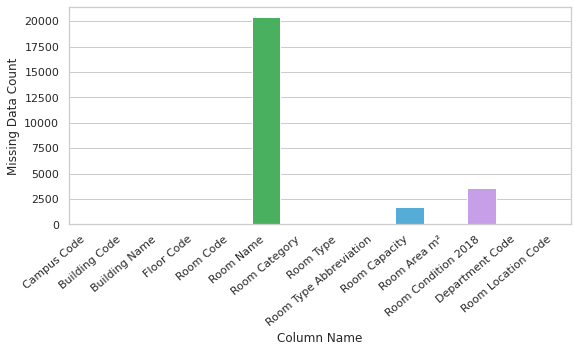
\includegraphics[width=0.5\textwidth]{resources/images/snap-9.png}
    \caption{Missing data summary of the timetable dataset}
    \label{timetable_data}
\end{figure}

% Data can be cleaned using two approaches as given below.
% \begin{enumerate}
%     \item Removing null values \label{app1}
%     \item Setting default values to the null values\label{app2}
% \end{enumerate}

% Approach \ref{app1}, is not feasible because removing all the \textit{Null} values, losses integrity of data.
% For example, \textit{UOM-SPACE-DATA} has 1 column that has more than 90\% null values, removing these values would mean deleting 90\% of data.  To avoid data integrity issues, default values for different data-types is used. For example, \textit{string/object} data type values are assigned \textit{\_missing\_} values and \textit{Integer/Float} values are assigned \textit{0/0.0} respectively.

% Once default values are set, we can analyse the columns that are relevant to the problem statement. If the columns are irrelevant, we can delete the concerned data columns. For example, \textit{Booking?} column is not related to the analysis.
% Another case is excluding the unnecessary/duplicate rows from the data, as seen in the timetable dataset, can be deleted. Also, options given as \textit{online option} for classes and \textit{off-site} option can be excluded.